\documentclass[letterpaper,12pt]{article}

\usepackage{amsmath}
\usepackage{amssymb,textcomp, esvect,esint}
\usepackage{amsthm}
\usepackage{graphicx,mathtools}
\usepackage{subcaption}
\usepackage[onehalfspacing]{setspace}
\usepackage{subfiles}
\usepackage{framed}
\usepackage{csvsimple}
\usepackage{booktabs}

\usepackage{tocvsec2}
%\usepackage[bookmarksdepth=subsection]{hyperref}
\usepackage[hidelinks]{hyperref}
\usepackage{bookmark}
\usepackage[margin=1in]{geometry}
\usepackage{authblk}
\usepackage{titling}
\setlength{\droptitle}{-1in}

\usepackage{mathrsfs,comment}

% place figures and tables where it seems like they should be
\usepackage{float}
\floatplacement{figure}{H}
\floatplacement{table}{H}
\usepackage{color}

\sloppy
\definecolor{lightgray}{gray}{0.5}
\setlength{\parindent}{0pt}

% automatically center figures/tables
\makeatletter
\g@addto@macro\@floatboxreset{\centering}
\makeatother


%%%%%%%%%%%%%%%%%%%%%%%%%%%%%%%%%%%%%%%%%%%%%%%%%%%%%%%%%%%%%%%%%%%%%%
% NEW COMMANDS
\newcommand{\bvec}[1]{\ensuremath{\mathbf{#1}}}

\newtheorem{theorem}{Theorem}
\newtheorem{proposition}{Proposition}
\newtheorem{definition}{Definition}

% section heading formatting
\renewcommand{\thesection}{\arabic{section}.}
\renewcommand{\thesubsection}{\thesection \arabic{subsection}}

\newenvironment{problem}[2][Problem]{\begin{trivlist}
\item[\hskip \labelsep {\bfseries #1}\hskip \labelsep {\bfseries #2.}]}{\end{trivlist}}
    
\newenvironment{solution}[2][Solution]{\begin{trivlist}
\item[\hskip \labelsep {\bfseries #1}\hskip \labelsep {\bfseries #2.}]}{\end{trivlist}}

\newenvironment{code}[2][Code]{\begin{trivlist}
\item[\hskip \labelsep {\bfseries #1}\hskip \labelsep {\bfseries #2.}]}{\end{trivlist}}

\usepackage{sectsty}
\usepackage{titlesec}
\sectionfont{\centering\fontsize{18pt}{1em}\selectfont}
\titlespacing*{\section}
{0pt}{15ex}{12ex}
\titlespacing*{\subsection}
{0pt}{10ex}{8ex}

\title{\fontsize{16pt}{1em}\bfseries Econ 712: Term Project}
\author{Leon Huetsch}


\begin{document}
\maketitle

\subsection*{1 Partial Equilibrium}
\subsubsection*{1.1 Recursive Problem of the Agent}
Bellman equation:
\begin{align*}
v(a,y) &= \max_{(c,a^{\prime})\ge 0} u(c) + \beta \sum_{y^{\prime} \in \mathcal{Y}} \pi \left(y^{\prime} | y \right) v(a^{\prime},y^{\prime}) \\
&\textit{s.t.} \ \ c + a^{\prime} = y + (1+r)a 
\end{align*}
where $\beta = \frac{1}{1+\rho}$ and $y^{\prime}$ follows an AR(1) process given by $\log(y^{\prime}) = \delta \log(y) + \sqrt{1-\delta^2} \varepsilon$ with $\varepsilon \sim N(0,\sigma_Y^2)$. \newline \newline
Plugging in the budget constraint yields the Bellman equation in one variable only.
\begin{align}
v(a,y) &= \max_{a^{\prime}\ge 0} u(y + (1+r)a - a^{\prime}) + \beta \sum_{y^{\prime} \in \mathcal{Y}} \pi \left(y^{\prime} | y \right) v(a^{\prime},y^{\prime})
\end{align}
First order condition withr respect to savings $a^{\prime}$ and the Envelope condition yield
\begin{align*}
u_c (y + (1+r)a - a^{\prime}) &= \beta \sum_{y^{\prime} \in \mathcal{Y}} \pi \left(y^{\prime} | y \right) v_1 (a^{\prime},y^{\prime}) \\
v_1 (a,y) &= u_c (y + (1+r)a - a^{\prime}) (1+r)
\end{align*}
Combining the two equations at the optimal asset holding decision $a^{\prime} (a,y)$ yields the stochastic Euler equation
\begin{equation}
u_c (y + (1+r)a - a^{\prime} (a,y)) = \beta \sum_{y^{\prime} \in \mathcal{Y}} \pi \left(y^{\prime} | y \right) u_c \left( y^{\prime} + (1+r) a^{\prime} (a,y) - a^{\prime} (a^{\prime} (a,y),y^{\prime}) \right) (1+r)
\end{equation}




\subsubsection*{1.2 Infinite Horizon VFI and Simulation}
The files VFI\_InfHorizon.m and Simulation\_InfiniteHorizon.m in the folder Part1\_PE/Functions/ contain the value function iteration and simulation for the infinite horizon case, respectively.



\subsubsection*{1.3 Finite Horizon VFI and Simulation}
The files VFI\_FinHorizon.m and Simulation\_FiniteHorizon.m in the folder Part1\_PE/Functions/ contain the value function iteration and simulation for the finite horizon case, respectively.




\subsubsection*{1.4 Infinite Horizon Case}
Figures 1 and 2 show the policy function for consumption in the infinite horizon case with low and high variance of the income process, respectively. \\
\begin{figure}
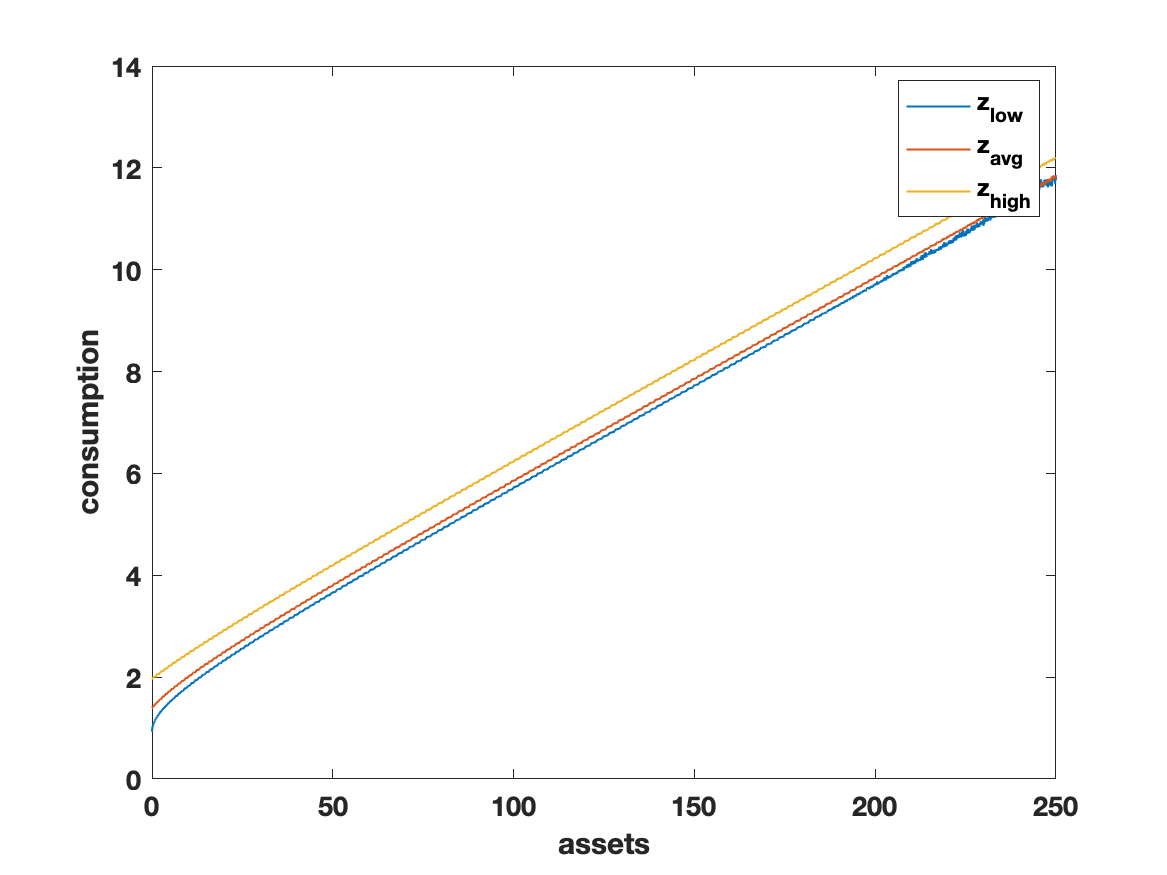
\includegraphics[scale=0.5]{Figures/Part1_PE/consFunc_inf_low}
\caption{Consumption function with low variance $\sigma_Y = 0.2$}
\end{figure}
As expected consumption increases with higher income, shown in the plot by an upward shift of the policy function for higher realizations of $z$. \\
\begin{figure}
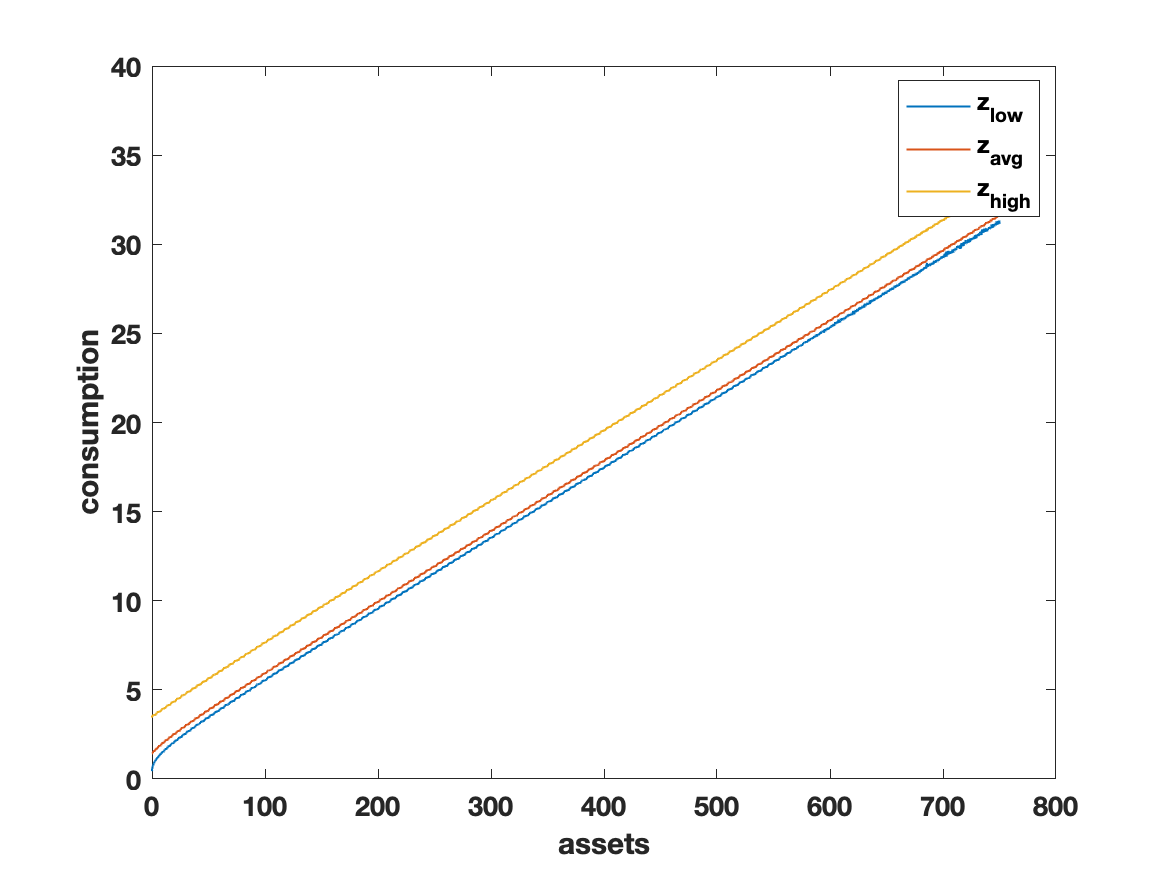
\includegraphics[scale=0.45]{Figures/Part1_PE/consFunc_inf_high}
\caption{Consumption function with high variance $\sigma_Y = 0.4$}
\end{figure}
With high income volatility consumption also increases with more income. The starker increase of consumption between income shocks here is due to the larger difference in levels of income shocks that comes from a higher variance. \\
The consumption function starts of concanve for low asset holdings as households consume most of any additional resources while it becomes more linear for high asset holdings.





\subsubsection*{1.5 Finite Horizon Case}
Figures 3 and 4 show the policy function for consumption in the finite horizon case for medium income with low and high variance of the income process, respectively. \\
\begin{figure}
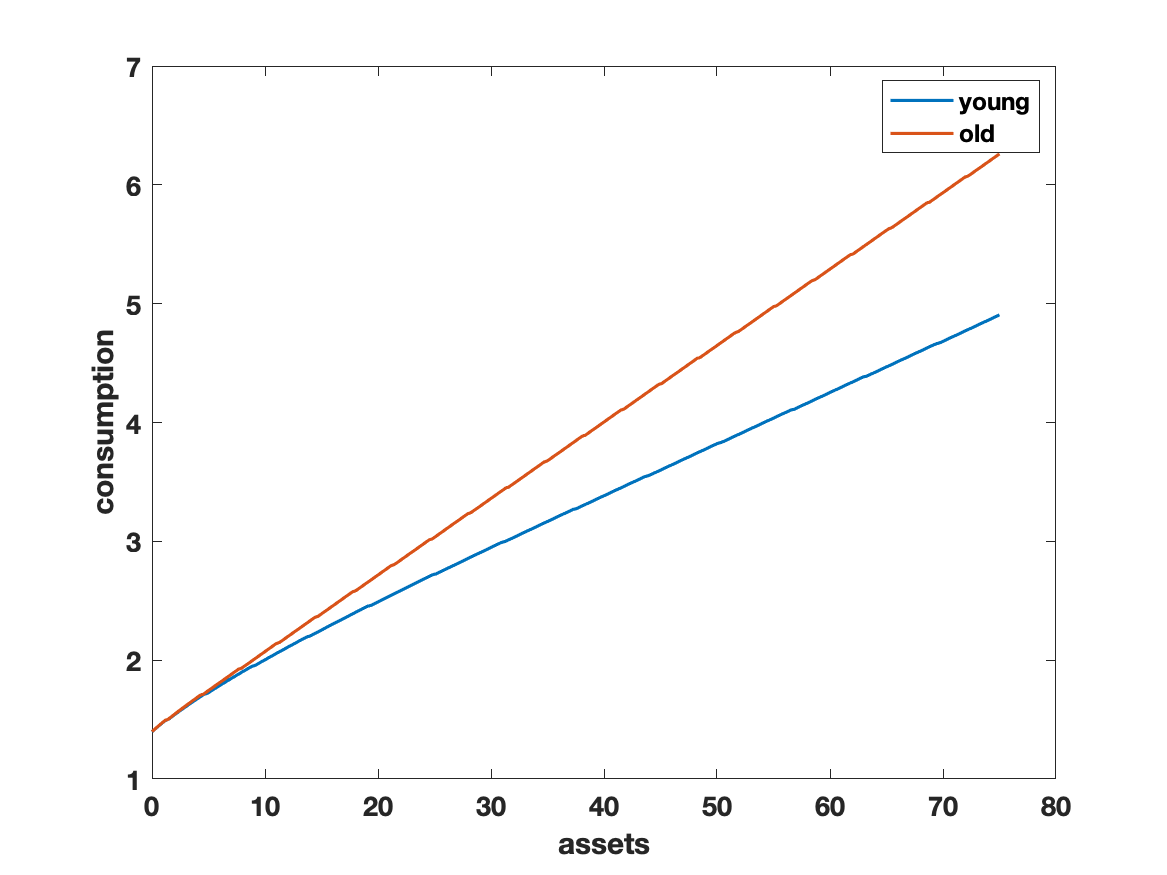
\includegraphics[scale=0.5]{Figures/Part1_PE/consFunc_fin_low}
\caption{Consumption function with low variance $\sigma_Y = 0.2$ and average income}
\end{figure}
Young households consume less and save more with the same available resources, as they face a longer lifespan and, thus, more future consumption periods which increases their precautionary savings motive. \\
\begin{figure}
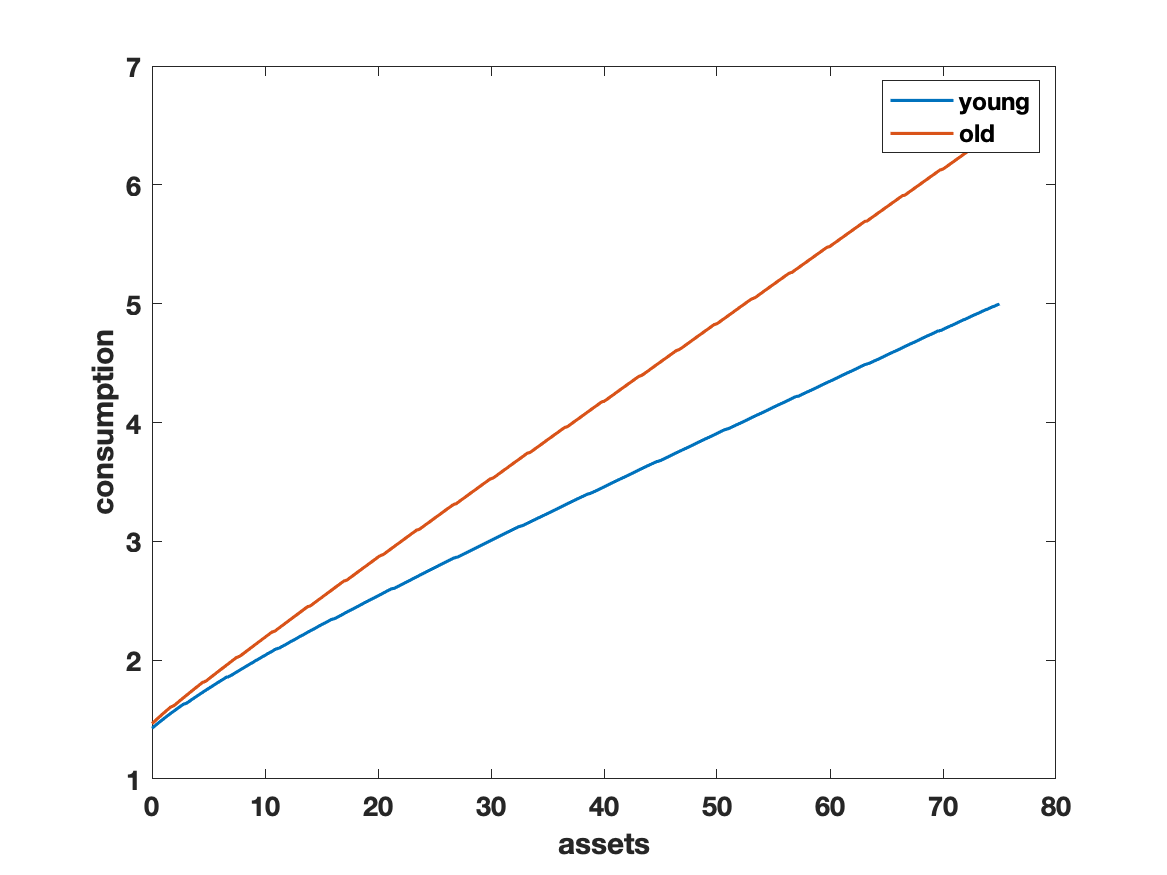
\includegraphics[scale=0.45]{Figures/Part1_PE/consFunc_fin_high}
\caption{Consumption function with high variance $\sigma_Y = 0.4$ and average income}
\end{figure}
The same holds true with high income volatility. Note that medium income is higher in the economy with high income volatility. \\
The consumption function of young households is also flatter, meaning the more assets they have the lower their consumption share compared to old households. As in the inifinite horizon case, consumption grows faster when asset holdings are low as households invest most of their additional resources in consumption when poor.

%Still the two plots are very similar in levels, which shows that the additional income is mostly invested into savings.




\subsubsection*{1.6 Hump in Life Cycle}
I simulated the economy with 10000 individuals over 61 periods and took the average consumption and asset holding paths. The parameters here are $\sigma_Y = 0.2$ and $\sigma = 1$. Figure 5 shows the resulting paths. \\

\begin{figure}
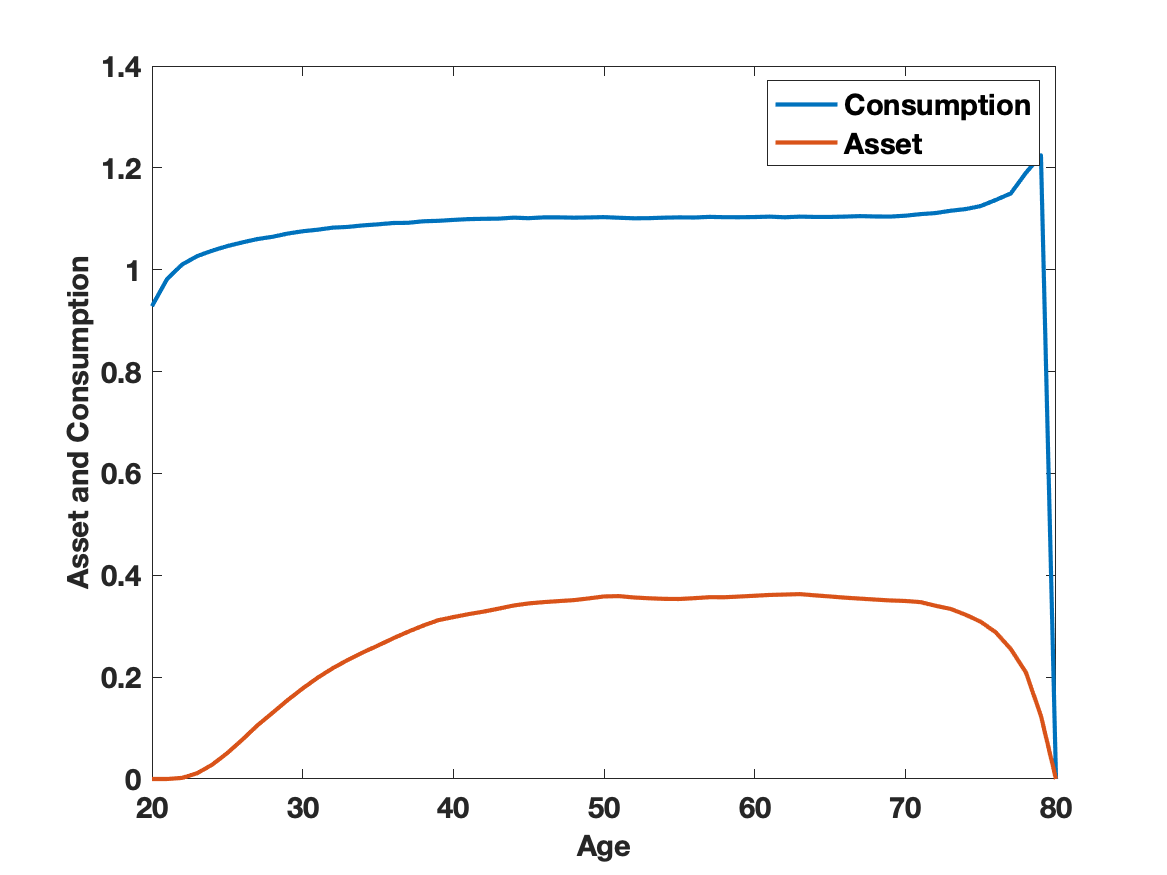
\includegraphics[scale=0.45]{Figures/Part1_PE/sim_simple}
\caption{Consumption and Assets over the life cycle}
\end{figure}

Figure 6 shors the consumption path over the life cycle for different risk aversion parameters. When households are more risk avers, they save more when young and, thus, consume less. In return they accumulate more assets that they get to consume later in life. 
Consumption is basically flat over the life cycle, households smooth consumption. They accumulate assets when young and dissave when old. \\ 

\begin{figure}
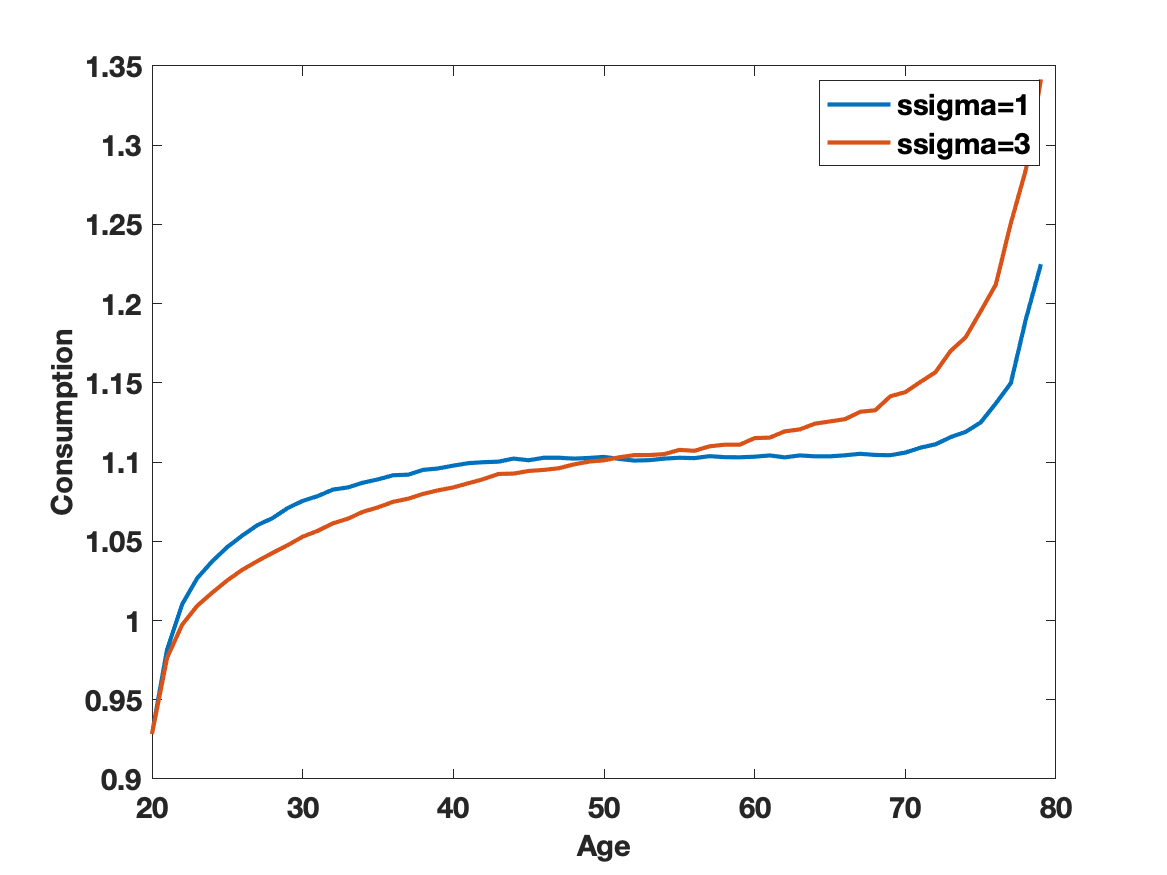
\includegraphics[scale=0.45]{Figures/Part1_PE/sim_risk}
\caption{Life cycle consumption for different risk aversion}
\end{figure}

The discount rate, $\rho = 0.04$, is larger than the interest rate, $r = 0.02$, thus, agents in principle would like to have a declining consumption profile. However, sice the borrowing constraint is set to $0$, this is not feasible as households cannot borrow when young and start off with zero assets. \\

\begin{figure}
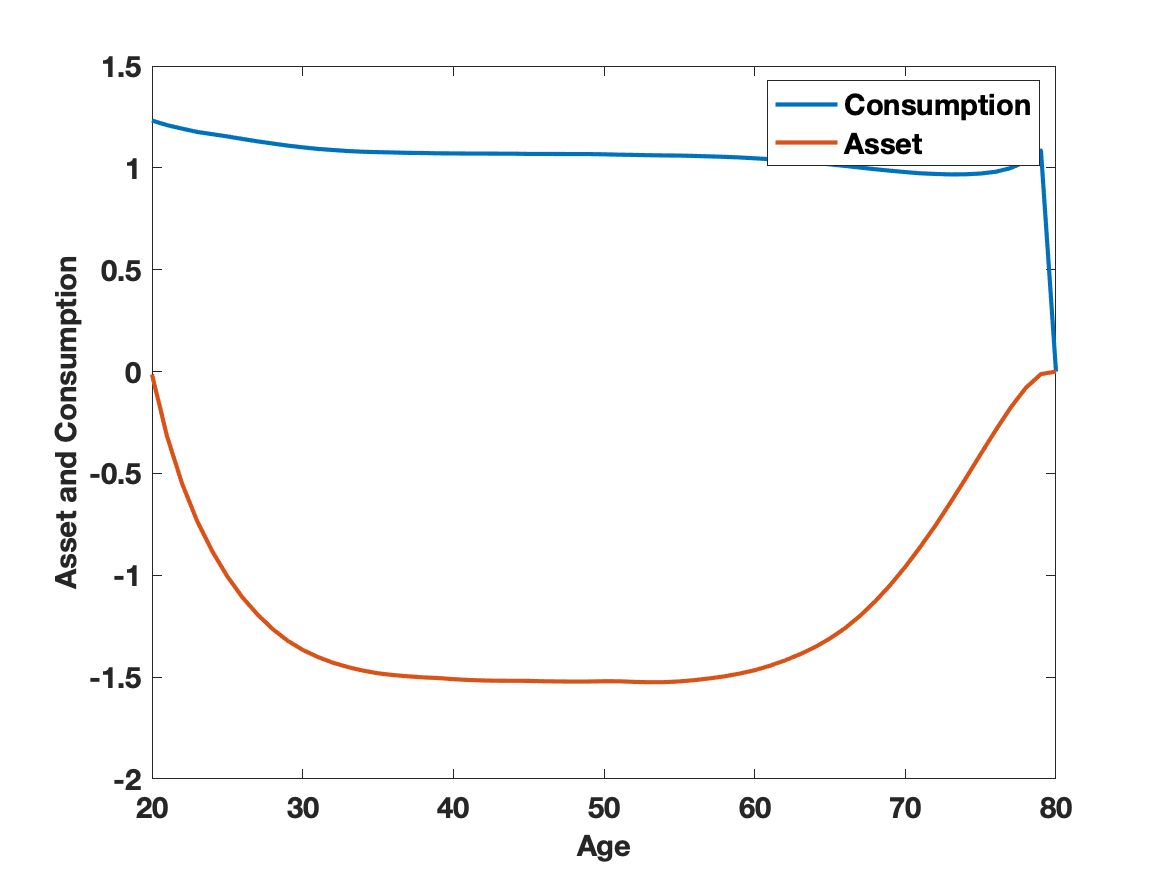
\includegraphics[scale=0.45]{Figures/Part1_PE/sim_borrowing}
\caption{Life cycle profile with relaxed borrowing constrait}
\end{figure}

Relaxing the borrowing constraint yields a declining consumption profile as shown in figure 6, though no hump. Households borrow when young as they start off with no assets and low income and pay back their debt towards the end of their life. Again, they chose a slightly declining consumption profile since the interest rate is too low to fully compensate their impatience.






\subsubsection*{1.7 Income and Mortality Data}
Adding mortality to the model increases the effective discount factor of households. However, mortality rates are close to zero when young, those they only really start mattering for old agents. Moreover, adding income data yields a hump shaped income profile. As a result agents would like to consume more when young, but cannot due to the borrowing constraing and low income. When getting older income increases and households consume the most in their middle age. There is less incentive for saving at that point because mortality rates start mattering and the effective discount factor decreases which yields a declining consumption profile when being old. 

\begin{figure}
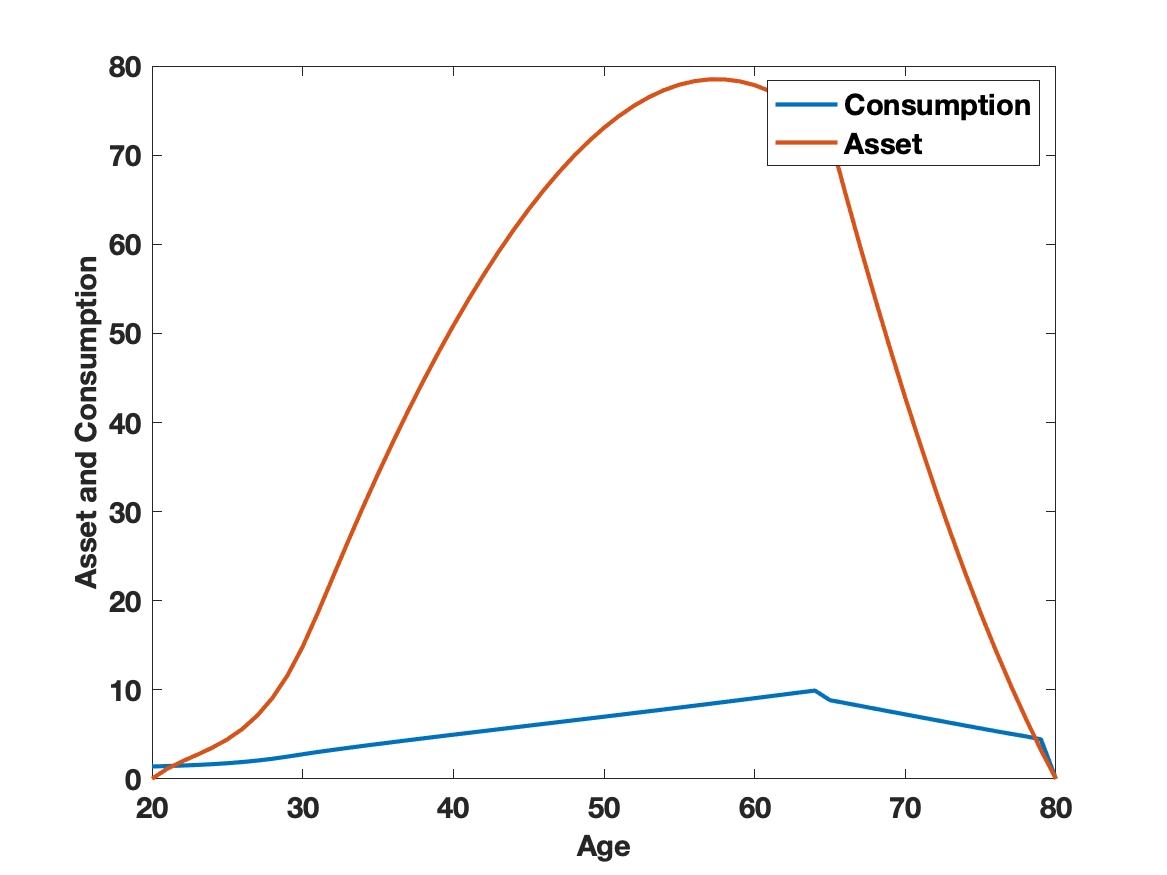
\includegraphics[scale=0.45]{Figures/Part1_PE/sim_Data}
\caption{Life cycle profile with Income and Mortality Data}
\end{figure}
\newpage





\subsubsection*{1.8 Empirical Life Cycle Profile Comparison}


I normalize consumption to the same initial level and still include the mortality and income data. As Figure 9 shows, the empirical life cycle model is a lot smoother. \\
\begin{figure}
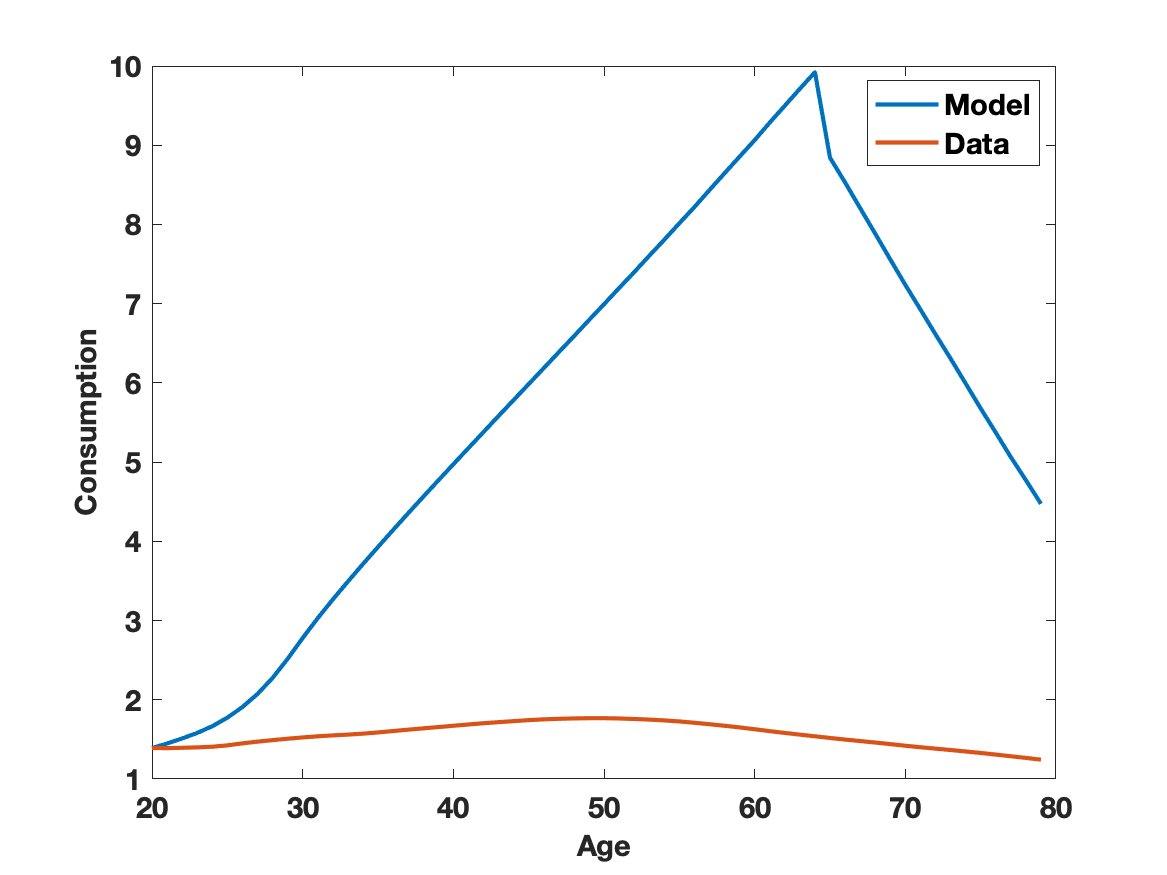
\includegraphics[scale=0.45]{Figures/Part1_PE/Data_comparison}
\caption{Life cycle profile Comparison with Data}
\end{figure}

One way to decrease the size of the hump is to reduce the precautionary savings motive, so households do not accumulate as many assets. Reducing the income process volatility to $\sigma_Y = 0.035$ results in a flatter consumption profile, closer to the empirical one. \\

\begin{figure}
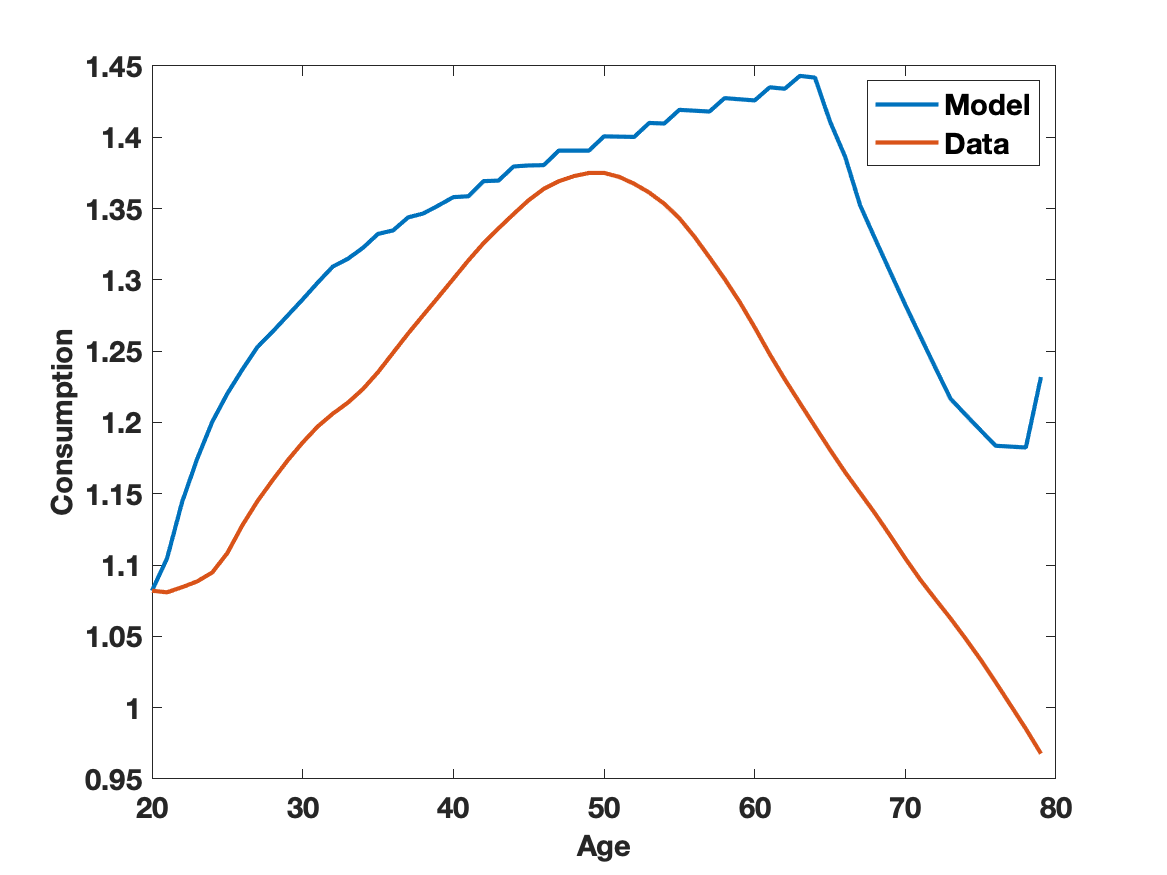
\includegraphics[scale=0.45]{Figures/Part1_PE/Data_comparison2}
\caption{Data comparison with less income volatility}
\end{figure}





\newpage
\subsection*{2 Gerneral Equilibrium}
\subsubsection*{2.1 Existence and Uniqueness of General Equilibrium}
I first solved for the general equilibrium with the highest risk aversion, persistence and volatility of the shock in order to check existence. \\
\begin{figure}
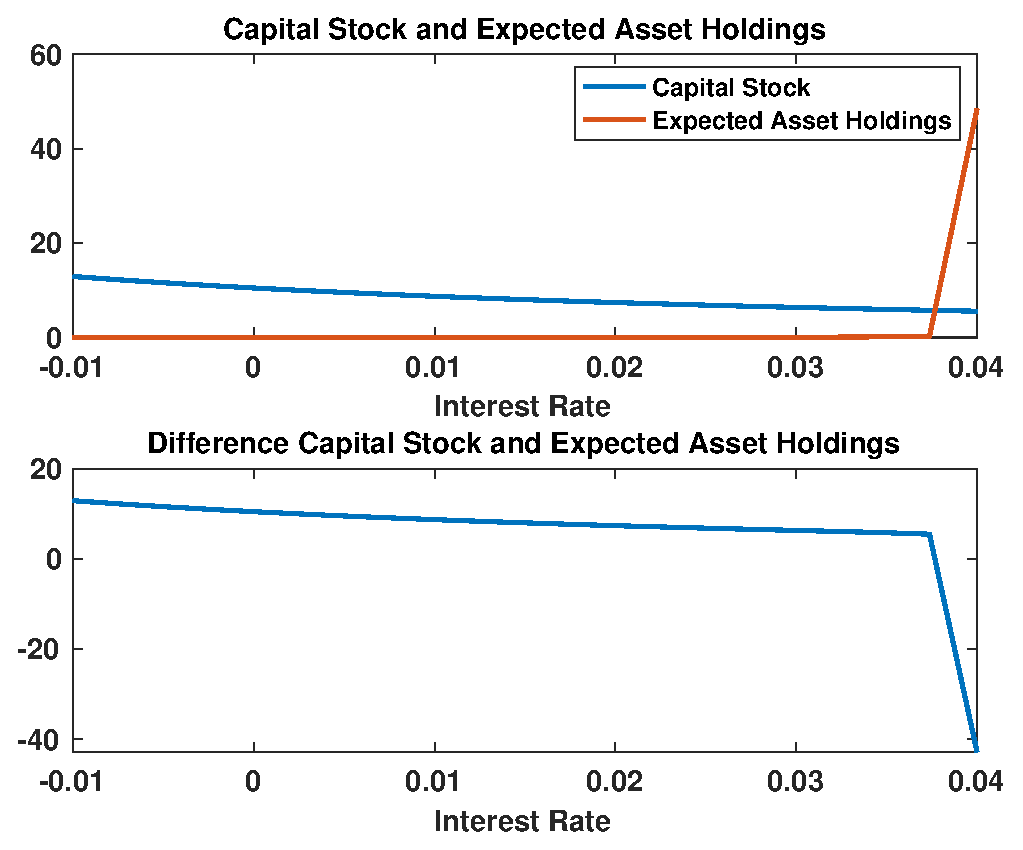
\includegraphics[scale=0.5]{Figures/Part2_GE/Capital_AssetHoldings}
\caption{Asset Holdings and Capital Demand as a Function of Interest Rate}
\end{figure}
Figure 5 shows that there exists a unique interest rate at which the capital market clears. The following plots show the associated stationary distribution for the equilibrium interest rate. \\
\begin{figure}
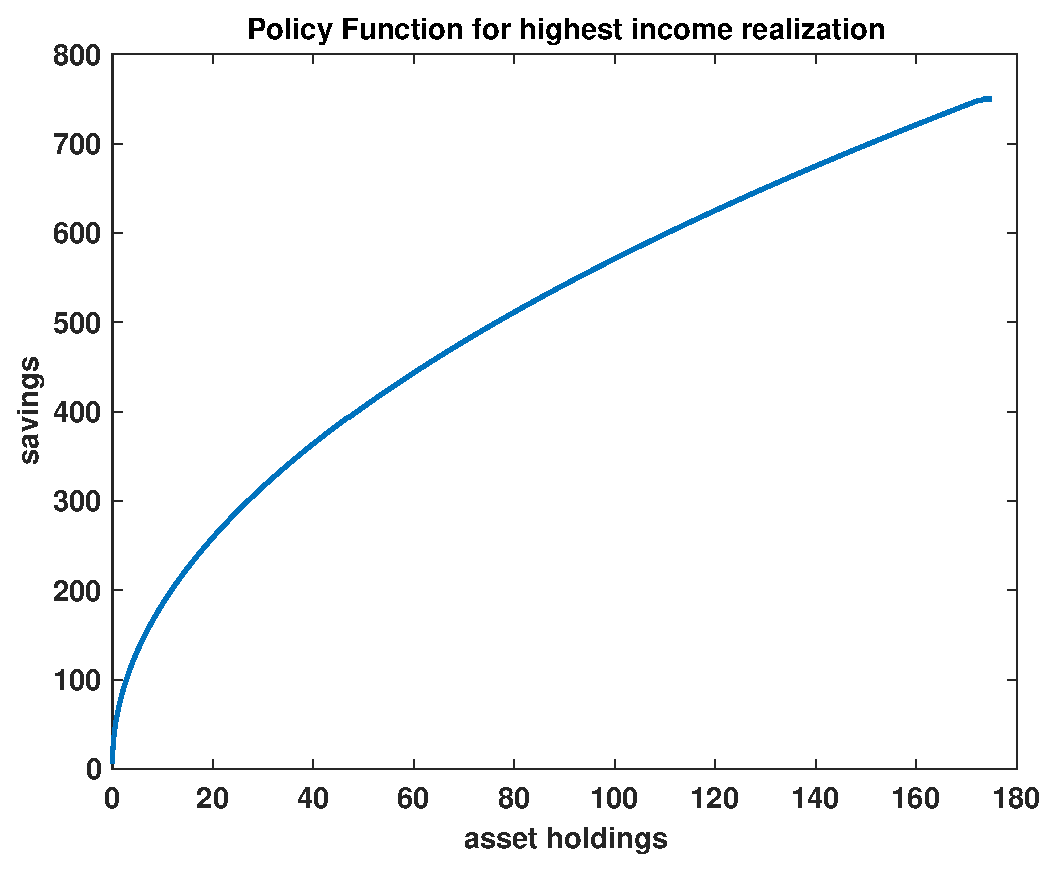
\includegraphics[scale=0.5]{Figures/Part2_GE/Policy_func_assets}
\caption{Policy Function for Assets}
\end{figure}
The policy function for assets at the highest income shock intersects with the 45 degree line, thus, the asset space can be bounded from above at the intersection as households will never go above that level of asset holdings if they start below. \\
\begin{figure}
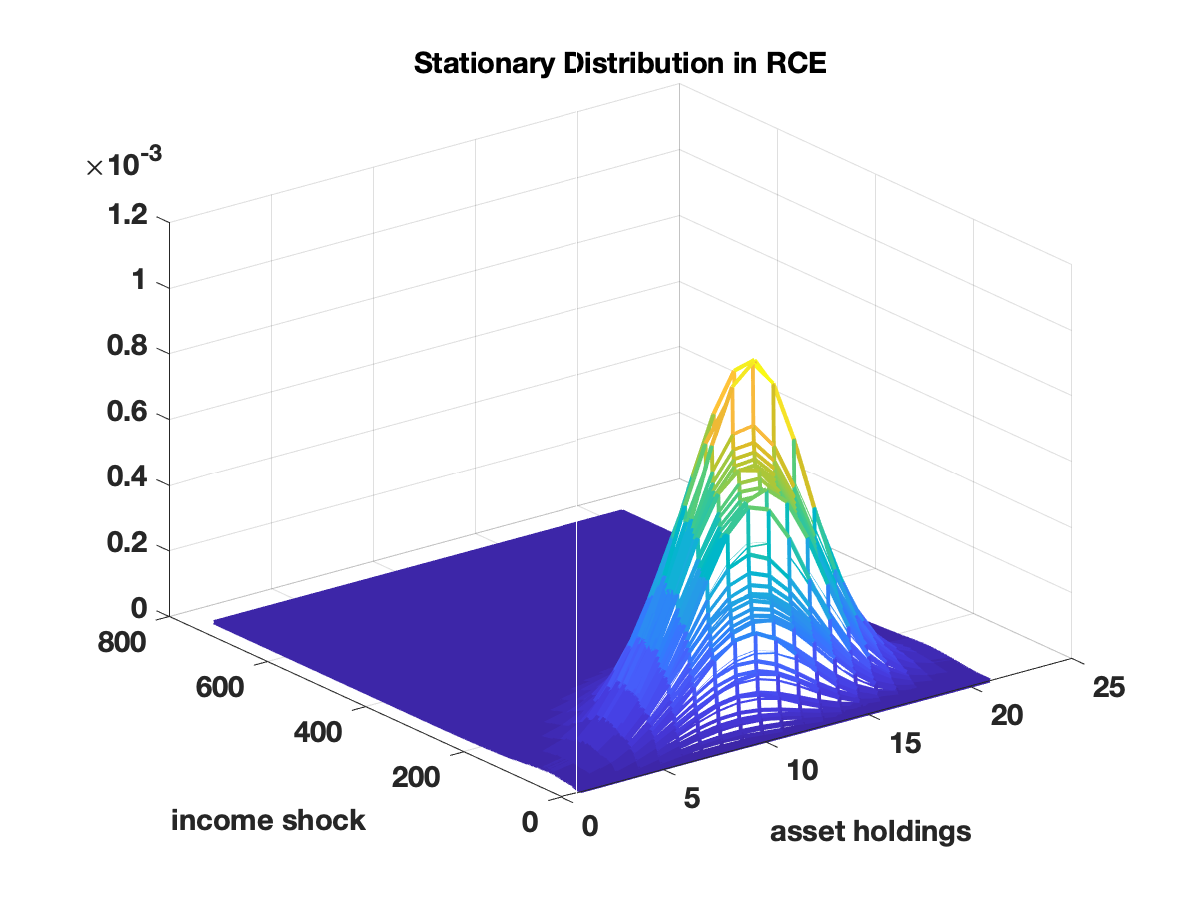
\includegraphics[scale=0.5]{Figures/Part2_GE/StationaryDist}
\caption{Stationary equilibrium Distribution}
\end{figure}




\newpage
\subsubsection*{2.2 Aiyagari's Table 2}
The following tables show the equilibrium interest rates for the different parameter specifications following Aiyagari's table 2 (1994).

\begin{table}
\begin{tabular}{llll}
\textbf{$\rho \setminus \sigma$} & \textbf{1} & \textbf{3} & \textbf{5} \\ \hline
\textbf{0.0}      & 4.1139       & 4.0106         & 3.9037        \\
\textbf{0.3}      & 4.0795       & 3.8872         & 3.6953        \\
\textbf{0.6}      & 4.0597       & 3.8117         & 3.5338        \\
\textbf{0.9}      & 3.9194       & 3.1122         & 2.1057       
\end{tabular}
\caption{Aiyagari Table 1: $\sigma_Y = 0.2$}
\end{table}

\begin{table}
\begin{tabular}{llll}
\textbf{$\rho \setminus \sigma$} & \textbf{1} & \textbf{3} & \textbf{5} \\ \hline
\textbf{0.0}      & 4.0833       & 3.8738         & 3.6490        \\
\textbf{0.3}      & 4.0514       & 3.7699         & 3.4781        \\
\textbf{0.6}      & 3.9653       & 3.5325         & 3.0600        \\
\textbf{0.9}      & 3.1943       & 0.7271         & -1.0802       
\end{tabular}
\caption{Aiyagari Table 1: $\sigma_Y = 0.4$}
\end{table}

The result is similar to Aiyagari's, particularly the comparative statics align well. The higher the idiosyncratic risk that households face, the larger the precautionary savings motive and, thus, the lower the equilibrium interest rate.







\subsubsection*{2.3 UBI}
The parametrization in the remainder of this question is 
\begin{align*}
&\sigma = 1 \\
&\delta = 0.8 \\
&\sigma_Y = 0.2
\end{align*}
For both economies, with and without UBI, a system of two equations in two unknowns has to be solved, however, the choice of variables and equations is over which to optimize is not unique. Importantly, the addition of a labor choice for households does not add an additional market clearing condition for labor with an additional variable of optimization. Since the aggregate production function is Cobb Douglas, only the ratio of capital to labor matters in the profit maximizing conditions of the firm, thus, capital and labor demand are not determined separately. The first order conditions for the firm show this in detail
\begin{align*}
r &= \alpha A \left( \frac{L}{K} \right)^{1-\alpha} - \delta \\
w &= \left( 1-\alpha \right) A \left( \frac{K}{L} \right)^\alpha 
\end{align*}
Isolating $K$ in the first equation and plugging it in the second yields
\begin{align*}
w = \left( 1-\alpha \right) A \left( \frac{\alpha A}{r + \delta} \right)^{\frac{\alpha}{1-\alpha}}
\end{align*}
Thus, the interest rate is a sufficient condition for wage as well as capital demand to labor demand ratio. Using this wage in the household problem for any given interest rate ensures labor market clearing. 

Then the interest rate has to chosen such that the capital market clears
\begin{align*}
E(a) = \left( \frac{\alpha A}{r + \delta} \right)^{\frac{1}{1-\alpha}} L_s
\end{align*}
$E(a)$ is expected asset holdings, meaning capital supply of the households next period. $L_s$ is effective labor supply of households, that is 
\begin{align*}
L_s = \int_{a,y} y l(a,y) d\phi(a,y)
\end{align*}
where $\phi$ is the stationary distribution. 

\paragraph{Without UBI: } I solve for the general equilibrium by finding the interest rate $r$ and disutility parameter $\kappa$ that clear the capital market and yield a labor participation rate of $80\%$. \\
Formally the conditions
\begin{align*}
E(a) &= \left( \frac{\alpha A}{r + \delta} \right)^{\frac{1}{1-\alpha}} L_s \\ 
0.8 &= \int_{a,y} l(a,y) d\phi(a,y)
\end{align*}
have to hold. \\

\paragraph{With UBI: } For Andrew Young's proposal I take the equilibrium $\kappa$ from the case without UBI and solve for the general equilibrium by finding the interest rate $r$ and tax rate $\tau$ such that the capital market and the government budget clears. \\
Formally the conditions
\begin{align*}
E(a) &= \left( \frac{\alpha A}{r + \delta} \right)^{\frac{1}{1-\alpha}} L_s \\ 
\lambda &= \tau w L_s = \tau w \int_{a,y} y l(a,y) d\phi(a,y)
\end{align*}
have to hold. \\


\subsubsection*{2.3.1 Results}
The following table shows macroeconomic aggregregates in the stationary distribution for both cases, with and without UBI.
 
\begin{table}
\begin{tabular}{@{}lccccc@{}}
\textbf{}                             & \multicolumn{1}{l}{\textbf{Output}} & \multicolumn{1}{l}{\textbf{Capital}} & \multicolumn{1}{l}{\textbf{Consumption}} & \multicolumn{1}{l}{\textbf{Wage}} & \multicolumn{1}{l}{\textbf{Interest\_Rate}} \\ \cmidrule(l){2-6} 
\textbf{Without UBI}                  & 1.6799                              & 4.2247                               & 1.4689                                   & 1.1849                            & 4.0430                                      \\
\multicolumn{1}{c}{\textbf{With UBI}} & 1.6177                              & 3.8045                               & 1.4374                                   & 1.1858                            & 4.0277                                     
\end{tabular}
\end{table}

\begin{figure}
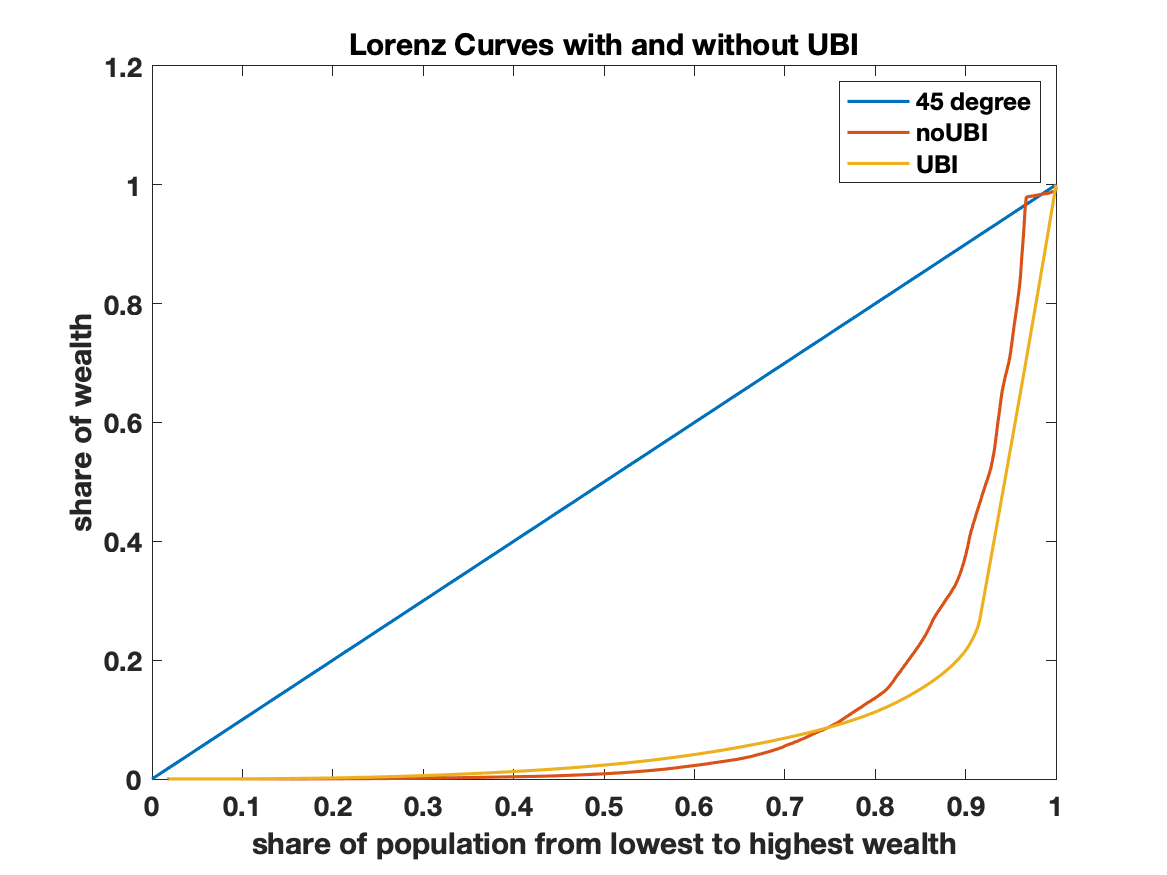
\includegraphics[scale=0.5]{Figures/Part2_UBI/Lorenz_Wealth}
\caption{Stationary equilibrium Distribution}
\end{figure}

\begin{figure}
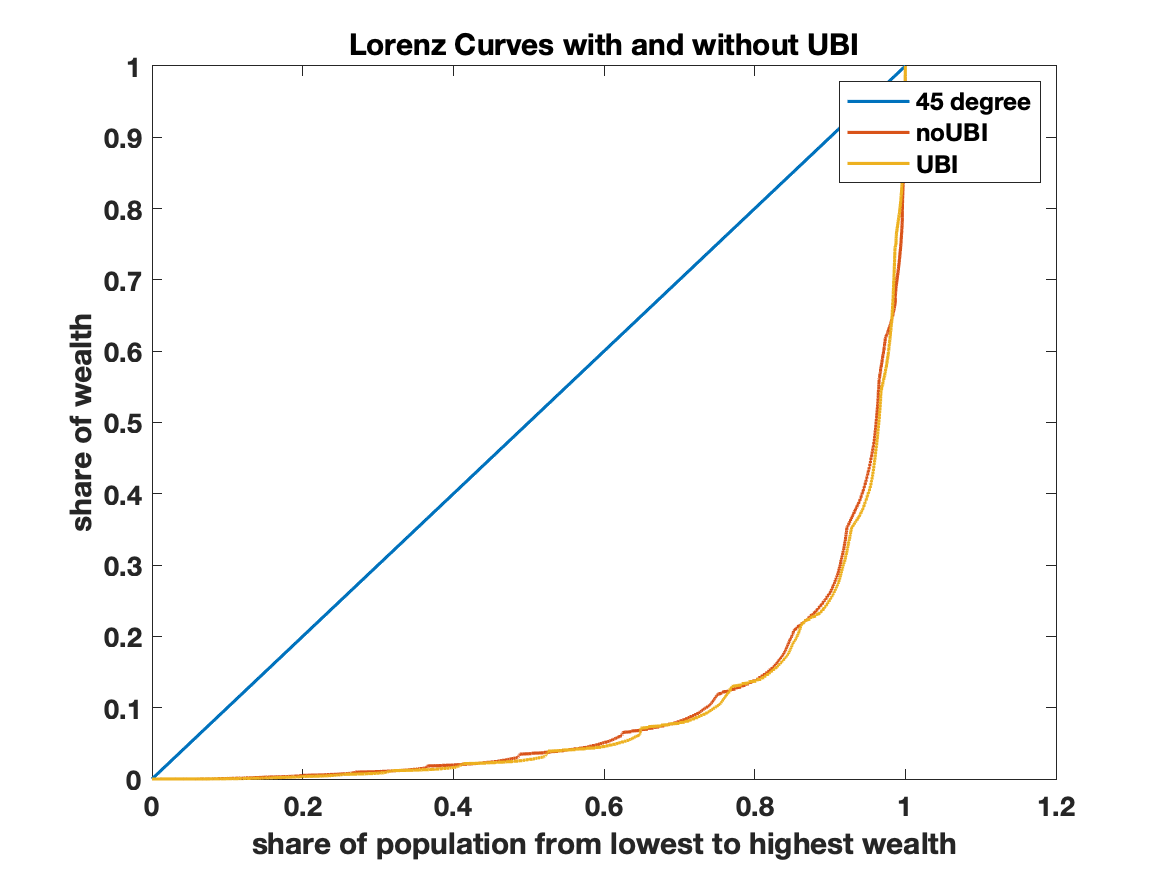
\includegraphics[scale=0.5]{Figures/Part2_UBI/Lorenz_Income}
\caption{Stationary equilibrium Distribution}
\end{figure}

The participation rate drops from 80\% without UBI to about 62\% after UBI is introduced due to the strong income effect of the unconditional UBI transfer. As a result wage stays almost the same although capital decreases. The interest rate declines slightly as the negative effect from the decrease in labor supply overpowers the positive effect from a reduction in capital on the marginal product of capital. As a result output as well as consumption decline after UBI is introduced. \\
Moreover, the Lorenz-Curve for the wealth distribution shows an increases in inequality through UBI. This is because labor participation went down and households that are not working will not accumulate assets. \\

The consumption equivalence variation is 
\end{document}